\documentclass[../main/main.tex]{subfiles}

\begin{document}

\section{Sphinx}

\subsection{Setup}

Using Sphinx requires only one simple Python package, \lstinline|sphinx|,
however, there also are other additional packages such as the
\lstinline|sphinx_rtd_theme| that we will install. 

\subsection{Quickstart}

We will use \lstinline|sphinx-quickstart| to quickly setup a Sphinx project
thereby gaining build files like a Makefile. For this project we need a vital
extension called \lstinline|autodoc|, thus we need enter \lstinline|y|, if we
are asked, whether we want to include it. 

The command should be entered in the root directory of the project, therefore
we will also enter \lstinline|docs| as the root path for the documentation, as
we do not want to mess up the source files with the documentation files. 

However, we can also enter the following commands, which will lead to the same
results: 

\begin{lstlisting}
sphinx-apidoc -o docs/ app/ -F -H Trackit -A Gary Ye -V 0.1
echo "sys.path.insert(0, os.path.abspath('../'))" >> docs/conf.py
\end{lstlisting}

\subsection{Generating the Documentation}

Sphinx works with \lstinline|*.rst| files, which can be seen as a script files,
in which we use a certain syntax to produce a certain documentation. 

However we can also use inline code documentation so that we don't have to
separate our source files from our documentation files by using the
\lstinline|autodoc| package. We merely have to write which kind of modules,
class, ..., have to be included in our documentation. As this can be a tedious
process to list them all, Sphinx has also included a helper script
\lstinline|sphinx-apidoc|, which we will use to generate the corresponding
\lstinline|rst| files. 

\begin{lstlisting}
>>> sphinx-apidoc -o docs app
Creating file docs/app.rst.
Creating file docs/app.crawling.rst.
Creating file docs/app.forms.rst.
Creating file docs/app.models.rst.
Creating file docs/app.models.facebook.rst.
Creating file docs/app.models.twitter.rst.
Creating file docs/app.views.rst.
Creating file docs/modules.rst.
\end{lstlisting}

To use \lstinline|autodoc| properly, it also needs to include the packages, thus
we need to set the \lstinline|PYTHONPATH| appropriately. In the
\lstinline|docs/conf.py|, we must also include the root directory of the project
into the \lstinline|PYTHONPATH|. 

\begin{lstlisting}[caption=docs/conf.py, label=lst:sphinxconfpy]
sys.path.insert(0, os.path.abspath('../'))
\end{lstlisting}

Basically, we can just enter the \lstinline|docs| directory now, and enter the
following \lstinline|make| command, in order to generate all files. 

\begin{lstlisting}
make html
\end{lstlisting}

\subsection{\lstinline|index.rst|}

For creating an aesthetic documentation tree, just use the following lines in
the \lstinline|index.rst| file: 

\begin{lstlisting}
.. toctree::
  :maxdepth: 2

  app
\end{lstlisting}

Where \lstinline|app| is the root module. A tree of \lstinline|maxdepth| = 2,
will be created recursively.  


\subsection{Read The Docs (optional)}
An extraordinary theme that guranteely gets you bonus points:

\begin{lstlisting}
pip install sphinx_rtd_theme
\end{lstlisting}

Find the line with \lstinline|html_theme|, and replace it with the following
three lines, provided in \ref{lst:sphinx_rtd}

\begin{lstlisting}[caption=docs/conf.py,label=lst:sphinx_rtd]
import sphinx_rtd_theme
html_theme = "sphinx_rtd_theme"
html_theme_path = [sphinx_rtd_theme.get_html_theme_path()]
\end{lstlisting}

The default theme should be \lstinline|alabaster|, however, a picture of the
Readthedocs theme should convince everyone. 

\begin{figure}
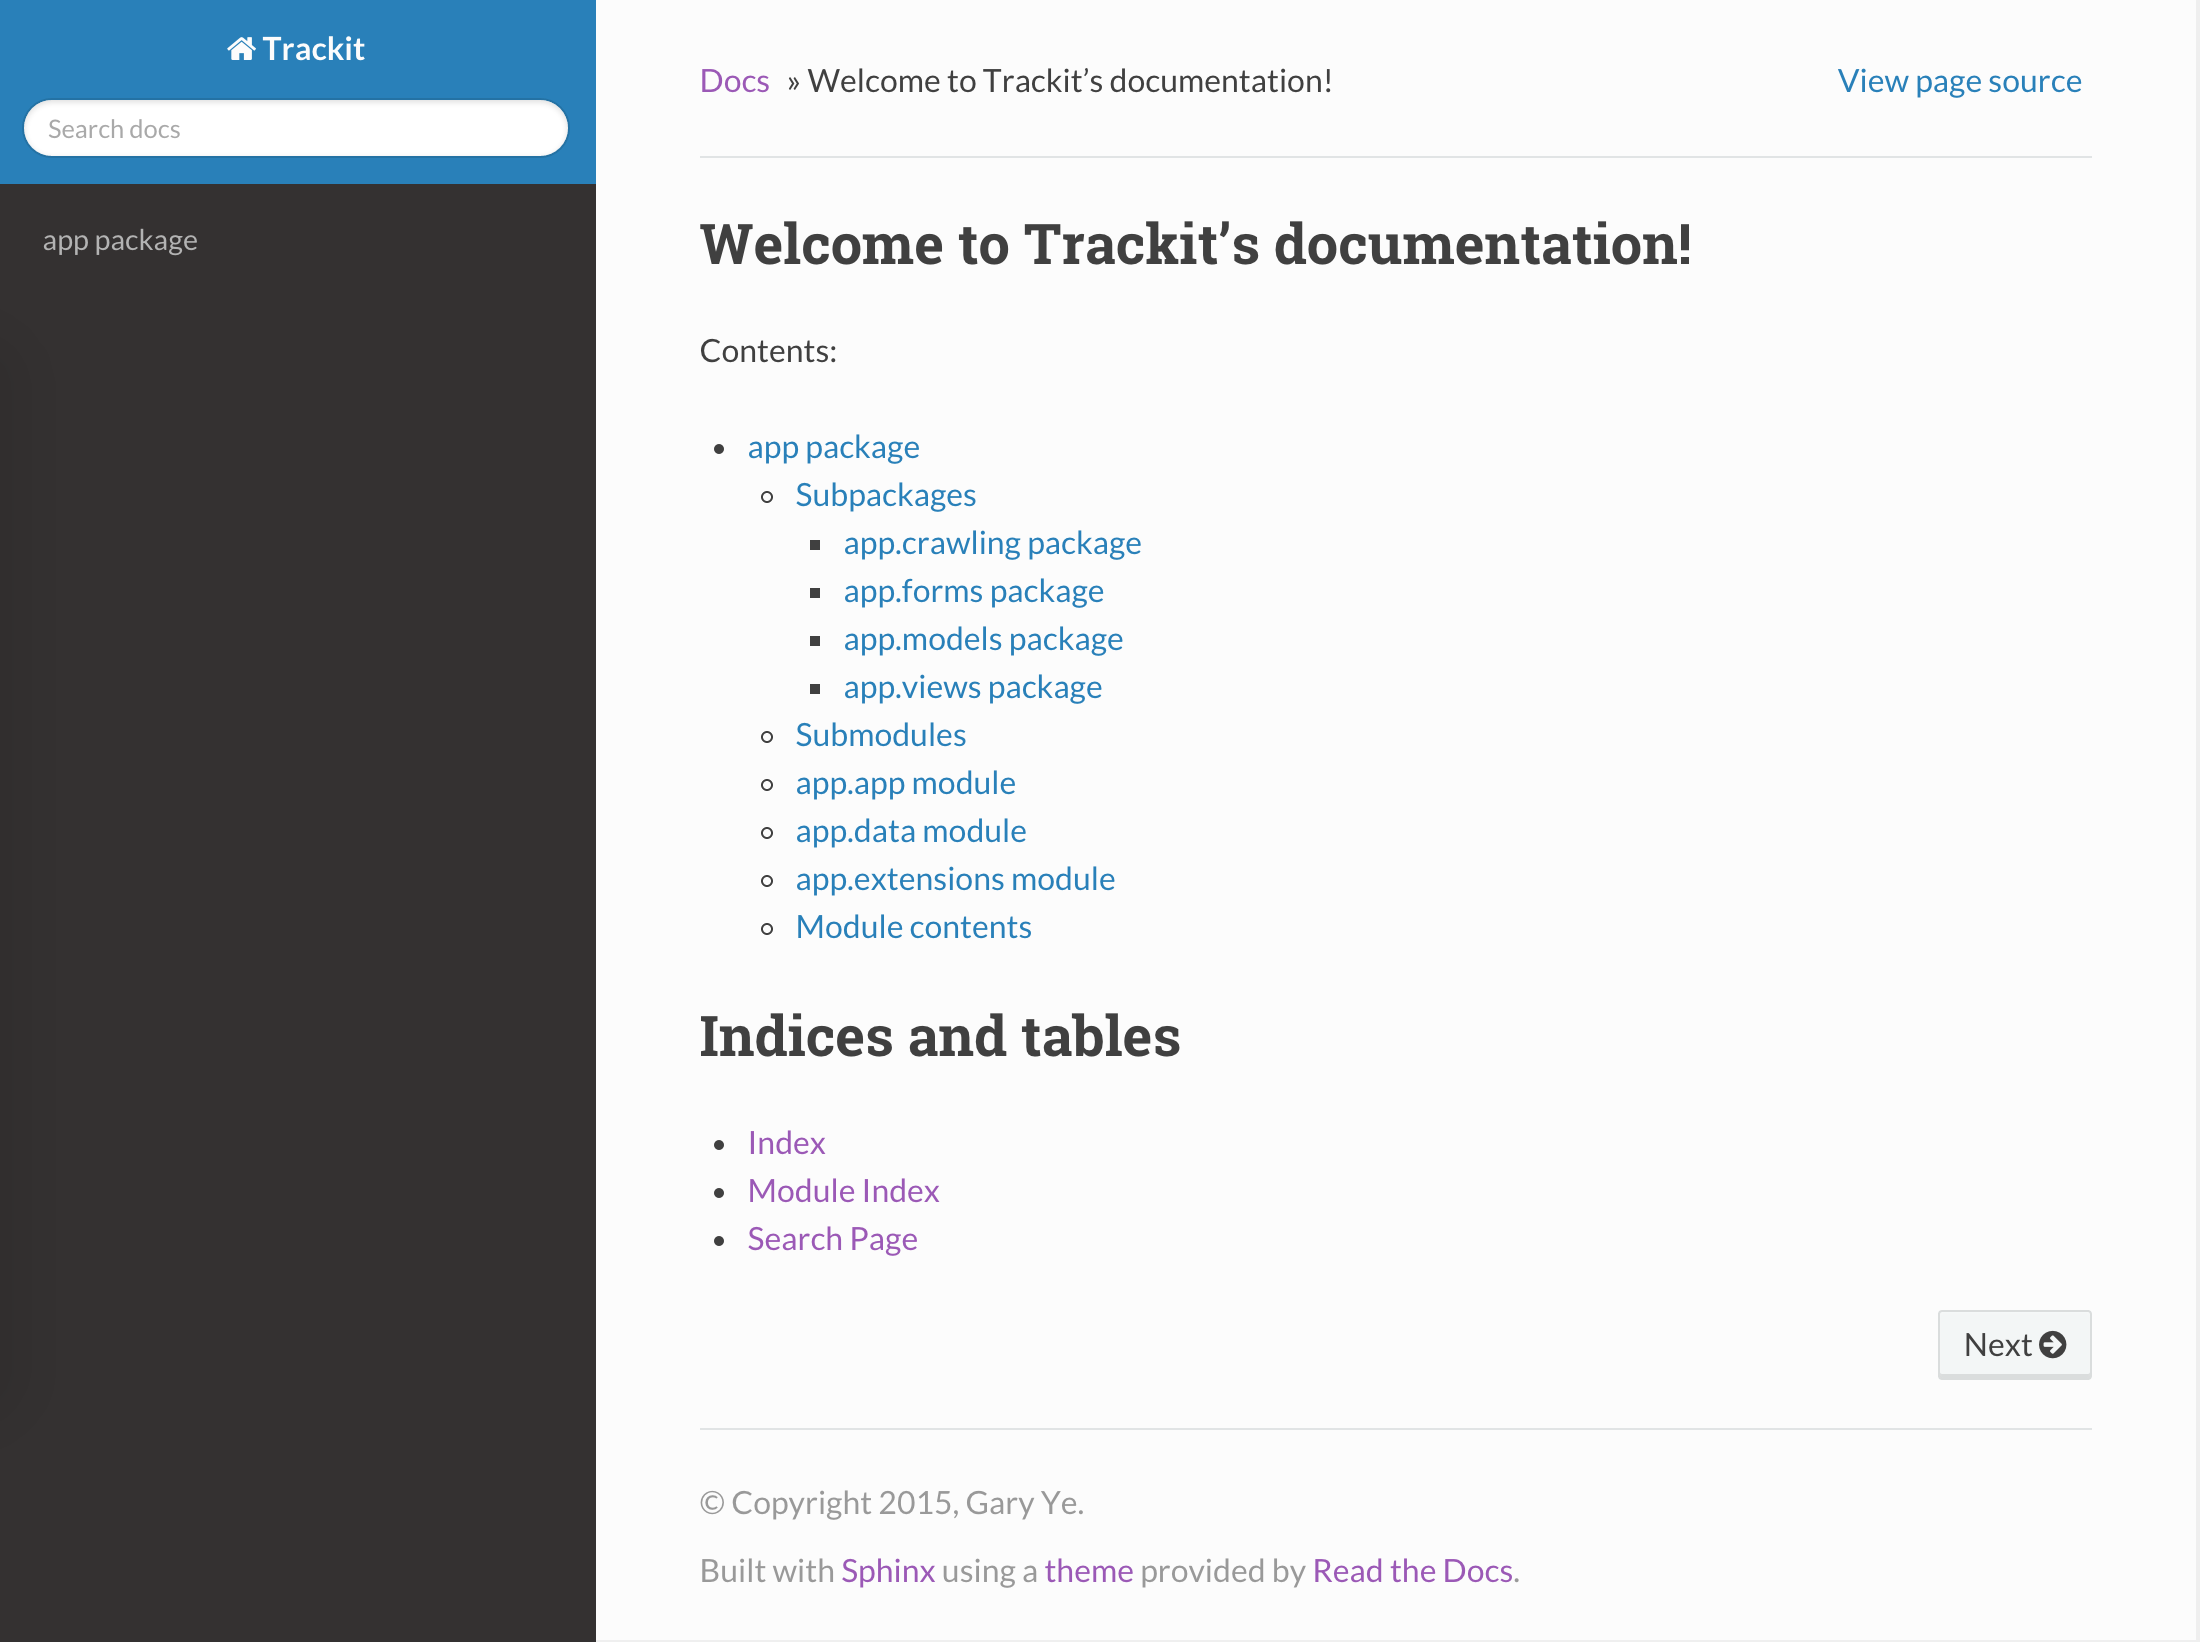
\includegraphics[]{../figures/rtd_sphinx.png}
\end{figure}

\subsection{Documentation Syntax}

The official way to document the code is provided in \cite{sphinx:python}.

\end{document}
